\documentclass[a4paper,12pt]{article} % тип документа
\usepackage{abraces}
\usepackage{mathtext}
\usepackage[T2A]{fontenc} % кодировка
\usepackage[utf8]{inputenc} % кодировка исходного текста
\usepackage[english,russian]{babel} % локализация и переносы
\usepackage{indentfirst}
\usepackage{hhline}
\usepackage{amsmath,amsfonts,amssymb,amsthm,mathtools}
\usepackage{wasysym}
\linespread{1,1}
\usepackage{geometry}
\usepackage{hyperref}
\usepackage{wrapfig}
\usepackage{fancyhdr}
\usepackage{caption}
\usepackage{multirow}
\geometry{
a4paper,
left=25mm,
top=25mm,
}
\usepackage{stackengine}
\stackMath

\setlength\abovecaptionskip{0.5\baselineskip}
\setlength\belowcaptionskip{0pt}
 
\def\@IEEEfigurecaptionsepspace{\vskip\abovecaptionskip\relax}%
\def\@IEEEtablecaptionsepspace{\vskip\abovecaptionskip\relax}%

\begin{document}

\begin{titlepage}
	\centering
	\vspace{5cm}
	{\scshape\LARGE Московский физико-технический институт \par}
	\vspace{4cm}
	{\scshape\Large Лабораторная работа \par}
	\vspace{1cm}
	{\huge\bfseries Определение энергии $\alpha$ - частиц по величине их пробега в воздухе \par}
	\vspace{1cm}
	\vfill
\begin{flushright}
	{\large выполнил студент 004 группы ФАКИ}\par
	\vspace{0.3cm}
	{\LARGE Михель Егор Александрович} \par

\end{flushright}
	
	\vfill

% Bottom of the page
\today
\end{titlepage}


%%%%%%%%%%%%%%%%%%%%%%%%%%%%%%%%%%%%%%%%%%%%%%%%%%%%%%%%%%%
\section{Цель работы}
\begin{itemize}
    \item Измерить пробег $\alpha$-частиц в воздухе тремя способами: с помощью торцевого счетчика Гейгера, синтиляционного счетчика и ионизационной камеры, по полученным данным определить энергию частиц.
    \item Не слишком огорчиться результатам.
\end{itemize}


\section{Теоретические положения}
При $\alpha$-распаде исходное ядро испускает $\alpha$-частицу (ядро гелия), в результате число протонов и нейтронов уменьшается на две единицы. Функциональная свзяь между энергией $\alpha$-частицы $E$ и периодом полураспада радиоактивного ядра $T_{1/2}$ описывается формулой
	\begin{equation*}
		 \lg T_{1/2} = \frac{a}{\sqrt{E}} + b.
	\end{equation*}
	
%%%%%%%%%%%%%%%%%%%%%%%%%%%%%%%%%%%%%%%%%%%%%%%%%%%%%%%%%%%%
\section{Экспериментальная установка}

\begin{wrapfigure}[13]{r}{0.4\textwidth}
    \centering
    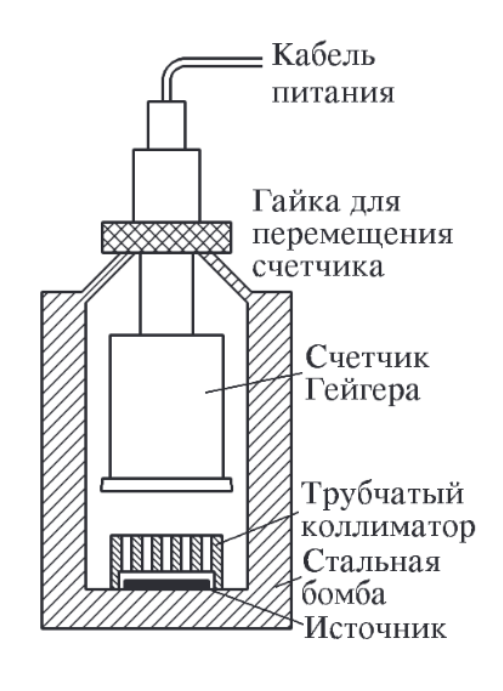
\includegraphics[width=0.35\textwidth]{Gayger.png}
    \caption{Установка для измерения пробега $\alpha$-частиц с помощью торцевого счетчика Гейгера}
    \label{fig:Geyger}
\end{wrapfigure}

В данной работе в качестве источника $\alpha$-частиц используется ${239}$Pu с периодом полураспада $T_{1/2} = 2,44 \cdot 10^4$ лет. Альфа-частицы, испускаемые ${239}$Pu состоят их трех моноэнергетических групп, различие между которыми лежит в пределах 50 кэВ. При той точности, которая достигается в наших опытах, их можно считать совпадающими по энергии, равной 5,15 МэВ.

Пробег $\alpha$-частиц в воздухе определяется треями способами:
	\begin{enumerate}
		\item
			С помощью счетчика Гейгера;
		\item
			C помощью сцинтилляционного счетчика;
		\item
			C помощью ионизационной камеры.
	\end{enumerate}
	
Счетчик Гейгера (\ref{fig:Geyger}) представляет собой газонаполненный конденсатор, который пробивается при пролёте ионизирующей частицы через объём газа.

\subsection{Исследование пробега $\alpha$-ч. счетчика Гейгера}	
Представим результаты измерений зависимости $N=N(x)$ в виде графика (\ref{graph::geiger}). 

\begin{figure}[h!]
	\centering
		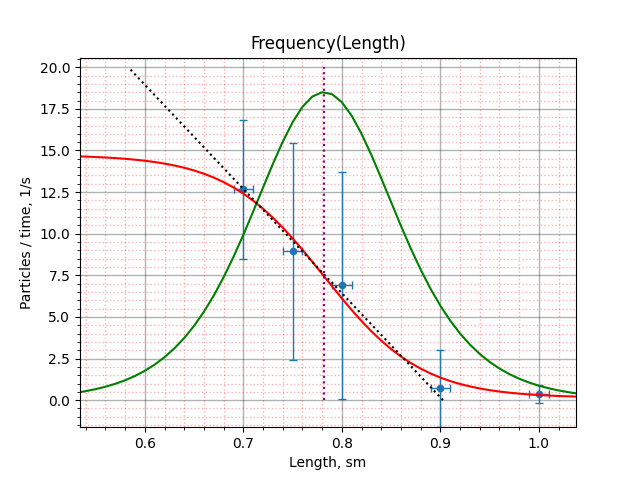
\includegraphics[width=1\textwidth]{ZoomedGeiger.png}
		\caption{График зависимости частоты от расстояния между счетчиком Гейгера и препаратом (приближенный).}
		\label{graph::geiger}
\end{figure}

\begin{figure}
    \begin{center}
    	\begin{tabular}{|c|c|c|c|c|}
    		\hline
    		$A_1$ & $A_2$ & $x_0$, мм & $dx$, мм \\ \hline
    		$14.7 \pm 0.3$  & $0.13 \pm 0.22$    & $0.782 \pm 0.006$        & $0.049 \pm 0.005$    \\ \hline
    	\end{tabular}
    	\caption{Параметры аппроксимации.}
    	\label{tab:pfrfmetry1}
    \end{center}
\end{figure}

%%%%%%%%%%%%%%%%%%%%%%%%%%%%%%%%%%%%%%%%%%%%%%%%%%%%%%%%%%%
\section{Вывод}

В ходе работы был измерен пробег $\alpha$-частицы в веществе тремя различными способами. По пробегу была оценена энергия частицы. Результаты методов не согласуются.

\end{document}
